% !Rnw root = learnR.Rnw




\marginnote{Read \margtt{c} as ``\underline{c}oncatenate'',
or perhaps as ``column''.\\[6pt]
\noindent Lists are widely used in R.  A data frame is a
special type of list,
used to collect together column objects under one name.}
\noindent
\fbox{\parbox{\textwidth}{\vspace*{-3pt}
\begin{tabular}{l}
{\bf Column Objects}\\
\qquad \txtt{width = c(11.3, 13.1, 20, 21.1, 25.8, 13.1)}\\[3pt]
\qquad \txtt{height = c(23.9, 18.7, 27.6, 28.5, 36, 23.4)}\\[4pt]
{\bf Data frame}\\
A data frame is a list of column objects, all of the same length.\\
\qquad \txtt{widheight <- data.frame( }\\
\qquad \qquad \txtt{width = c(11.3, 13.1, 20, 21.1, 25.8, 13.1),}\\
\qquad \qquad \txtt{height = c(23.9, 18.7, 27.6, 28.5, 36, 23.4)}\\
\qquad \txtt{ )}\\[4pt]
{\bf Also:} Arithmetic operations; simple plots; input of data.\\
\end{tabular}
\vspace*{-3pt}}}
\vspace*{3pt}

\section{Practice with R commands}
\marginnote{The R language has the standard abilities for evaluating
arithmetic and logical expressions.  There are numerous functions
that extend these basic arithmetic and logical abilities.}
Try the following
\begin{Schunk}
\begin{Sinput}
2+3        # Simple arithmetic
\end{Sinput}
\begin{Soutput}
[1] 5
\end{Soutput}
\begin{Sinput}
1:5        # The numbers 1, 2, 3, 4, 5
\end{Sinput}
\begin{Soutput}
[1] 1 2 3 4 5
\end{Soutput}
\begin{Sinput}
mean(1:5)  # Average of 1, 2, 3, 4, 5
\end{Sinput}
\begin{Soutput}
[1] 3
\end{Soutput}
\begin{Sinput}
sum(1:5)   # Sum of 1, 2, 3, 4, 5
\end{Sinput}
\begin{Soutput}
[1] 15
\end{Soutput}
\begin{Sinput}
(8:10)^2   # 8^2 (8 to the power of 2), 9^2, 10^2
\end{Sinput}
\begin{Soutput}
[1]  64  81 100
\end{Soutput}
\end{Schunk}

In addition to \txtt{log()}, note \txtt{log2()} and \txtt{log10()}:
\marginnote{A change by a factor of 2 is a one unit change
  on a log2 scale. A change by a factor of 10 is a one unit change
  on a log10 scale.}
\begin{Schunk}
\begin{Sinput}
log2(c(0.5, 1, 2, 4, 8))
\end{Sinput}
\begin{Soutput}
[1] -1  0  1  2  3
\end{Soutput}
\begin{Sinput}
log10(c(0.1, 1, 10, 100, 1000))
\end{Sinput}
\begin{Soutput}
[1] -1  0  1  2  3
\end{Soutput}
\end{Schunk}
\noindent
It turns out, surprisingly often, that logarithmic scales are
appropriate for one or other type of graph.  Logarithmic scales focus
on relative change --- by what factor has the value changed?

The following uses the relational operator \txtt{$>$}:
\marginnote{
Other relational operators are\\
\margtt{$<\quad >=\quad <\quad <=\quad ==\quad !=$}
}
\begin{Schunk}
\begin{Sinput}
(1:5) > 2  # Returns FALSE FALSE  TRUE  TRUE  TRUE
\end{Sinput}
\begin{Soutput}
[1] FALSE FALSE  TRUE  TRUE  TRUE
\end{Soutput}
\end{Schunk}

\subsection*{Demonstrations}

Demonstrations can be highly helpful in learning to use R's functions.
The following are some of demonstrations that are available for
graphics functions:
\begin{marginfigure}
Images and perspective plots:
\begin{Schunk}
\begin{Sinput}
demo(image)
demo(persp)
\end{Sinput}
\end{Schunk}
\end{marginfigure}
\begin{Schunk}
\begin{Sinput}
demo(graphics)   # Type <Enter> for each new graph
library(lattice)
demo(lattice)
\end{Sinput}
\end{Schunk}

\begin{marginfigure}For the following, the {\em vcd} package must be installed:
\begin{Schunk}
\begin{Sinput}
library(vcd)
demo(mosaic)
\end{Sinput}
\end{Schunk}
\end{marginfigure}

Especially for \txtt{demo(lattice)}, it pays to stretch the graphics
window to cover a substantial part of the screen.  Place the cursor on
the lower right corner of the graphics window, hold down the left
mouse button, and pull.

The following lists available demonstrations:
\begin{Schunk}
\begin{Sinput}
## List demonstrations in attached packages
demo()
## List demonstrations in all installed packages
demo(package = .packages(all.available = TRUE))
\end{Sinput}
\end{Schunk}

\section{A Short R Session}\label{ss:shortR}
We will work with the data set shown in Table
\ref{tab:travel}:

% latex table generated in R 3.0.1 by xtable 1.7-1 package
% Sat Jul 20 10:40:12 2013
\begin{table*}[ht]
\centering
\begin{tabular}{rrrrrrl}
  \hline
 & thickness & width & height & weight & volume & type \\
  \hline
Aird's Guide to Sydney & 1.30 & 11.30 & 23.90 & 250 & 351 & Guide \\
  Moon's Australia handbook & 3.90 & 13.10 & 18.70 & 840 & 955 & Guide \\
  Explore Australia Road Atlas & 1.20 & 20.00 & 27.60 & 550 & 662 & Roadmaps \\
  Australian Motoring Guide & 2.00 & 21.10 & 28.50 & 1360 & 1203 & Roadmaps \\
  Penguin Touring Atlas & 0.60 & 25.80 & 36.00 & 640 & 557 & Roadmaps \\
  Canberra - The Guide & 1.50 & 13.10 & 23.40 & 420 & 460 & Guide \\
   \hline
\end{tabular}
\vspace*{15pt}

\caption{Weights and volumes, for six Australian travel
books.}\label{tab:travel}
\end{table*}

\subsection*{Entry of columns of data from the command line}
The following enters data as numeric vectors:
\marginnote{Read \margtt{c} as
  ``\underline{c}oncatenate'', or perhaps as
  ``column''.  It joins elements together into a vector, here
  numeric vectors.}
\begin{Schunk}
\begin{Sinput}
volume <- c(351, 955, 662, 1203, 557, 460)
weight <- c(250, 840, 550, 1360, 640, 420)
\end{Sinput}
\end{Schunk}

Now store details of the books in the character vector \txtt{description}:
\marginnote{The end result is that objects \margtt{volume}, \margtt{weight}
and \margtt{description} are stored in the workspace.}
\begin{Schunk}
\begin{Sinput}
description <- c("Aird's Guide to Sydney",
 "Moon's Australia handbook",
 "Explore Australia Road Atlas",
 "Australian Motoring Guide",
 "Penguin Touring Atlas", "Canberra - The Guide")
\end{Sinput}
\end{Schunk}

\subsection*{Listing the workspace contents}

Use \txtt{ls()} to examine the current contents
of the workspace.
\begin{Schunk}
\begin{Sinput}
ls()
\end{Sinput}
\begin{Soutput}
[1] "description" "volume"      "weight"     
\end{Soutput}
\end{Schunk}
Use the argument \txtt{pattern} to specify a search pattern:
\begin{marginfigure}[40pt]
Note also:\\[-5pt]
\begin{Schunk}
\begin{Sinput}
ls(pattern="^des")
  ## begins with 'des'
ls(pattern="ion$")
  ## ends with 'ion'
\end{Sinput}
\end{Schunk}
\end{marginfigure}
\begin{Schunk}
\begin{Sinput}
ls(pattern="ume")   # Names that include "ume"
\end{Sinput}
\begin{Soutput}
[1] "volume"
\end{Soutput}
\end{Schunk}

\subsection*{Operations with numeric \txtt{vectors}}
Here are the values of \txtt{volume}
\begin{Schunk}
\begin{Sinput}
volume
\end{Sinput}
\begin{Soutput}
[1]  351  955  662 1203  557  460
\end{Soutput}
\end{Schunk}

To extract the final element of \txtt{volume}, do:
\begin{Schunk}
\begin{Sinput}
volume[6]
\end{Sinput}
\begin{Soutput}
[1] 460
\end{Soutput}
\end{Schunk}
For the ratio of weight to volume, i.e., the density, we can do:
\begin{Schunk}
\begin{Sinput}
weight/volume
\end{Sinput}
\begin{Soutput}
[1] 0.7123 0.8796 0.8308 1.1305 1.1490 0.9130
\end{Soutput}
\end{Schunk}

\subsection*{A note on functions}

For the \txtt{weight/volume} calculation, two decimal places in the output
is more than adequate accuracy. The following uses the function
\txtt{round()} to round to two decimal places:
\begin{marginfigure}[24pt]
More simply, type:
\begin{Schunk}
\begin{Sinput}
round(weight/volume, 2)
\end{Sinput}
\end{Schunk}
Providing the arguments are in the defined
order, they can as here be omitted from
the function call.
\end{marginfigure}
\begin{Schunk}
\begin{Sinput}
round(x=weight/volume, digits=2)
\end{Sinput}
\begin{Soutput}
[1] 0.71 0.88 0.83 1.13 1.15 0.91
\end{Soutput}
\end{Schunk}

\marginnote[11pt]{Many functions, among them \margtt{plot()} that is used
  for Figure \ref{fig:denplot}, accept unnamed as well as named
  arguments. The symbol `\margtt{\ldots}' is used to denote the possibility of
  unnamed arguments.}  Functions take {\em arguments} --- these supply
data on which they operate.  For \txtt{round()} the arguments are
`\txtt{x}' which is the quantity that is to be rounded, and
`\txtt{digits}' which is the number of decimal places that should
remain after rounding.

\marginnote[12pts]{If a `\txtt{\ldots}' appears, indicating that there can
be unnamed arguments, check the help page for details.}
Use the function \txtt{args()} to get details of the named
arguments:
\begin{Schunk}
\begin{Sinput}
args(round)
\end{Sinput}
\begin{Soutput}
function (x, digits = 0) 
NULL
\end{Soutput}
\end{Schunk}

\subsection*{Tabulation}
Use the function \texttt{table()} for simple numeric tabulations,
thus:
\begin{Schunk}
\begin{Sinput}
type <- c("Guide","Guide","Roadmaps","Roadmaps",
          "Roadmaps","Guide")
table(type)
\end{Sinput}
\begin{Soutput}
type
   Guide Roadmaps 
       3        3 
\end{Soutput}
\end{Schunk}

\subsection*{A simple plot}
Figure \ref{fig:denplot} plots \txtt{weight} against \txtt{volume},
for the six Australian travel books.  Note the use of the graphics
formula \verb!weight ~ volume! to specify the $x-$ and
$y-$variables. It takes a similar from to the ``formulae'' that are
used in specifying models, and in the functions \txtt{xtabs()} and
\txtt{unstack()}.
\begin{marginfigure}
\begin{Schunk}


\centerline{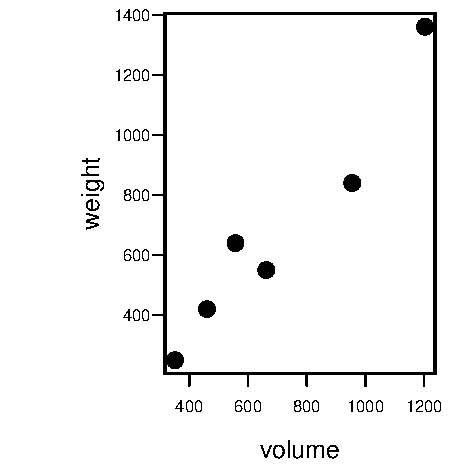
\includegraphics[width=0.98\textwidth]{../figs/02-denplot-1} }

\end{Schunk}
 \caption{Weight versus volume, for six Australian travel
books.}\label{fig:denplot}
\end{marginfigure}

Code for Figure \ref{fig:denplot} is:
\begin{Schunk}
\begin{Sinput}
## Code
plot(weight ~ volume, pch=16, cex=1.5)
  # pch=16: use solid blob as plot symbol
  # cex=1.5: point size is 1.5 times default
## Alternative
plot(volume, weight, pch=16, cex=1.5)
\end{Sinput}
\end{Schunk}

% To plot \txtt{(weight} against \txtt{volume} (Figure
% \ref{fig:denplot}), type one of the following:

The axes can be labeled:
\begin{Schunk}
\begin{Sinput}
plot(weight ~ volume, pch=16, cex=1.5,
     xlab="Volume (cubic mm)", ylab="Weight (g)")
\end{Sinput}
\end{Schunk}

Interactive labeling of points \marginnote{Use \margtt{text()} for
  non-interactive labeling of points.}  (e.g., with species names) can
be done interactively, using \txtt{identify()}:
\begin{Schunk}
\begin{Sinput}
identify(weight ~ volume, labels=description)
\end{Sinput}
\end{Schunk}
Then click the left mouse button above or below a point, or on the
left or right, depending on where you wish the label to appear.
Repeat for as many points as required.

On most systems, the labeling can be terminated by clicking the right
mouse button.  On the Windows GUI, an alternative is to click on the
word ``Stop'' that appears at the top left
of the screen, just under ``Rgui'' on the left of the blue panel
header of the R window. Then click on ``Stop locator''.

\subsection*{Formatting and layout of plots}
There are extensive abilities that may be used to control
the formatting and layout of plots, and to add features such as
special symbols, fitted lines and curves, annotation (including
mathematical annotation), colors, \ldots

\section{Data frames -- Grouping columns of data}\label{sec:df}

\marginnote{Data frames are pervasive in R. Most datasets that are
  included with R packages are supplied as data frames.}
\fbox{\parbox{\textwidth}{
\begin{tabular}{ll}
  Data frames & Store data that have a cases by
columns layout.\\[6pt]
  Creating & Enter from the command line (small datasets)\\
  data frames & Or: Use \txtt{read.table()} to input from a file.\\[6pt]
Columns of & \txtt{travelbooks\$weight} or \txtt{travelbooks[, 4]}\\
data frames & or \txtt{travelbooks[, "weight"]}\\
\end{tabular}
}}
\vspace*{8pt}

The following code groups the several columns of Table
\ref{tab:travel} together, under the name \txtt{travelbooks}.  It is
tidier to have matched columns of data grouped together into a data
frame, rather than separate objects in the workspace.
\marginnote[9pt]{The vectors \margtt{weight}, \margtt{volume}
  and \margtt{description} were entered earlier, and (unless subsequently
  removed) can be copied directly into the data frame.\\[6pt]
It is a matter of convenience whether the description
information is used to label the rows, or alternatively placed in a
column of the data frame.}
{\small
\begin{Schunk}
\begin{Sinput}
## Group columns together into a data frame
travelbooks <- data.frame(
   thickness = c(1.3, 3.9, 1.2, 2, 0.6, 1.5),
   width = c(11.3, 13.1, 20, 21.1, 25.8, 13.1),
   height = c(23.9, 18.7, 27.6, 28.5, 36, 23.4),
   weight = weight,  # Use values entered earlier
   volume = volume,  # Use values entered earlier
   type = c("Guide", "Guide", "Roadmaps", "Roadmaps",
            "Roadmaps", "Guide"),
   row.names = description
)
## Remove objects that are not now needed.
rm(volume, weight, description)
\end{Sinput}
\end{Schunk}
}

\subsection*{The storage of character data as factors}
\marginnote{While in most contexts factors and character vectors are
  interchangeable, there are important exceptions.}
Vectors of character, such as \txtt{type}, are by default stored in
the data frame as {\em factors}.  In the data as stored,
\txtt{"Guide"} is 1 and \txtt{"Roadmaps"} is 2. Stored with the factor
is an attribute table that interprets 1 as \txtt{"Guide"} and 2 as
\txtt{"Roadmaps"}.

\subsection*{Accessing the columns of data frames}

\marginnote[12pt]{For a matrix or array, users are restricted to
the first and second of these alternatives.  With a matrix
\margtt{travelmat} use, e.g., \margtt{travelmat[,4]} or
\margtt{travelmat[,"weight"]}.}
The following are alternative ways to extract the column
\txtt{weight} from the data frame:
{\small
\begin{Schunk}
\begin{Sinput}
travelbooks[, 4]
travelbooks[, "weight"]
travelbooks$weight
travelbooks[["weight"]]   # Reference as a list.
\end{Sinput}
\end{Schunk}
}
%$

There are several mechanisms that avoid repeated
reference to the name of the data frame.
The following are alternative ways to plot \txtt{weight} against \txtt{volume}:
\begin{itemizz}
\item[]{\em 1. Use the parameter \txtt{data},
\marginnote{Most modeling functions and many plotting functions accept a
\margtt{data} argument.}
where available, in
the function call}\\[-2pt]
\begin{Schunk}
\begin{Sinput}
plot( weight ~ volume, data=travelbooks)
\end{Sinput}
\end{Schunk}
\item[]{\em 2. Use \txtt{with()}: Take columns from specified
data frame}\\[-2pt]
\begin{Schunk}
\begin{Sinput}
## Take columns from the specified data frame
with(travelbooks, plot(weight ~ volume))
\end{Sinput}
\end{Schunk}
\vspace*{-3pt}

\noindent
\end{itemizz}
Both these mechanisms look first for a data frame column with a needed
name. The workspace is searched only if this fails.

\begin{marginfigure}[84pt]
Attachment of a data frame:
\begin{Schunk}
\begin{Sinput}
attach(travelbooks)
plot( weight ~ volume)
detach(travelbooks)
 ## Detach when no longer
 ## required.
\end{Sinput}
\end{Schunk}
\end{marginfigure}
A third option, usually best avoided,
is to use \txtt{attach()} to add the data frame to the search list. In
this case, names in the workspace take precedence over column names in
the attached data frame -- not usually what is wanted if there are
names in common.

Subsection \ref{ss:moreattach} will discuss the attaching of packages
and image files.

\section{Input of Data from a File}\label{sec:input}

The function \txtt{read.table()} is designed for input from a
rectangular file into a data frame. There are several variants on this
function --- notably \txtt{read.csv()} and \txtt{read.delim()}.

\marginnote[12pt]{This use of \margtt{datafile()}, avoiding
  use of the mouse to copy the file and the associated need
  to navigate the file system, is a convenience for teaching
  purposes.}  First use the function \txtt{datafile()}
(\textit{DAAG}) to copy from the {\em DAAG} package and into the
working directory a data file that will be used for demonstration purposes.

\begin{Schunk}
\begin{Sinput}
## Place the file in the working directory
## NB: DAAG must be installed
DAAG::datafile("travelbooks")
\end{Sinput}
\end{Schunk}
\noindent
Use \txtt{dir()} to check that the file is indeed in the working directory:
\begin{Schunk}
\begin{Sinput}
dir(pattern="travel")
  # File(s) whose name(s) include 'travel'
\end{Sinput}
\end{Schunk}

The first two lines hold the column headings and first row, thus:\vspace*{9pt}

\noindent
{
\begin{tabular}{rrrrrrl}
\hline
 & thickness & width & height & weight & volume & type \\
\hline
Aird's Guide to Sydney & 1.30 & 11.30 & 23.90       & 250 &  351 &    Guide \\
. . .
\end{tabular}
}
\vspace*{3pt}

\noindent Observe that column 1, which has the row names, has no name.

The following reads the file into an R data frame:
\marginnote{
Row 1 has column names.\\
\noindent
Column 1 has row names.
}
\begin{Schunk}
\begin{Sinput}
## Input the file to the data frame travelbooks
travelbooks <- read.table("travelbooks.txt",
                          header=TRUE, row.names=1)
\end{Sinput}
\end{Schunk}
The assignment places the data frame in the workspace, with the name
\txtt{travelbooks}.  The first seven columns are numeric.  The
character data in the final column is by default stored as a factor.

\paragraph{Data input -- points to note:}

\begin{itemizz}
\item [-] Alternatives to command line input include the
  R Commmander menu and the RStudio menu.  These make it
  easy to check that data are being correctly entered.
\item[-] If the first row of input gives column names, specify
  \txtt{heading=TRUE}.  If the first row of input is the first row of
  data, specify \txtt{heading=FALSE}.
\item[-] See \txtt{help(read.table)} for details of parameter
  settings that may need changing to match the data format.
  \marginnote[-0.5cm]{Section \ref{sec:entry} discusses
    common types of input errors.}
\item[-] Character vectors that are included as columns in data frames
  become, by default, factors.  \marginnote[-0.5cm]{Character vectors
    and factors can often, but by no means always, be treated as
    equivalent.}
\end{itemizz}

\section{Sources of Help}\label{sec:workinghelp}

\marginnote[12pt]{Note also:\\
\margtt{help.search()}\\
\margtt{apropos()}\\
\margtt{help.start()}\\
\margtt{RSiteSearch()}
}
\noindent
\begin{framed}
\vspace*{-10pt}
\begin{Schunk}
\begin{Sinput}
help()           # Help for the help function
help(plot)       # Show the help page for plot
?plot            # Shorthand for help(plot)
example(plot)    # Run examples from help(plot)
demo()           # List available demonstrations
vignette()       # Get information on vignettes
                 # NB also browseVignettes()
\end{Sinput}
\end{Schunk}
\vspace*{-10pt}
\end{framed}

\noindent
This section enlarges on the very brief details in Subsection \ref{ss:ch1-help}

\subsection*{Access to help resources from a browser screen}
Type \txtt{help.start()} to display a screen that gives a browser
\marginnote{Official R manuals include \underline{An Introduction to
    R}, a manual on \underline{Writing R Extensions}, and so on.}
interface to R's help resources.  Note especially
\underline{Frequently Asked Questions} and \underline{Packages}.
Under \underline{Packages}, click on \underline{base} to get
information on base R functions. Standard elementary statistics
functions are likely to be found under \underline{stats}, and base
graphics functions under \underline{graphics}.

Also available, after clicking on a package name, is a link
\underline{User guides, package vignettes and other documentation.}
Click to get details of any documentation that is additional to the
help pages.

\subsection*{Searching for key words or strings}

Use \txtt{help.search()} to look for functions that include a specific
word or part of word in their alias or title. Thus,
functions for operating on character strings are likely to have
\marginnote{By default, all installed packages are
searched.  Limiting the search, here to \txtt{package="base"},
will often give more manageable and useful output.}
``str'' or ``char'' in their name. Try
\begin{Schunk}
\begin{Sinput}
help.search("str", package="base")
help.search("char", package="base")
\end{Sinput}
\end{Schunk}

The function \txtt{RSiteSearch()} searches web-based resources, including
R mailing lists, for the text that is given as argument.

\subsection*{Examples that are included on help pages}

All functions have help pages.  Most help pages include\marginnote{To
  work through the code for an example, look on the screen for the
  code that was used, and copy or type it following the command line
  prompt. Or get the code from the help page.} examples, which can be
run using the function \txtt{example()}.  Be warned that, even for
relatively simple functions, some of the examples may illustrate
non-trivial technical detail.

\subsection*{Vignettes}

\marginnote[12pt]{Vignettes are created from a Markdown or HTML or
  LaTeX document in which R code is embedded, surrounded by
  markup that controls what is to be done with the code and with any
  output generated.  See Chapter \ref{ch:rstudio}.}  Many packages
have vignettes; these are typically pdf or (with version $\ge$ 3.0.0
of R) HTML files that give information on the package or on specific
aspects of the package. To get details of vignettes that are available
in a package, call \txtt{browseVignettes()} with the package name (as
a character string) as argument.  Thus, for the \textit{knitr}
package, enter \txtt{browseVignettes(package="knitr")}.

The browser window that appears will list the vignettes, with the
option to click on links that, in most cases, offer a choice of
one of \underline{PDF} and \underline{HTML}, \underline{source},
and \underline{R code}.

\subsection*{Searching for Packages}

A good first place to look, for information on packages that relate to
one or other area of knowledge, is the R Task Views web page, at:
\url{http://cran.r-project.org/web/views/}. See also the website
\url{http://crantastic.org/}, which has details on what packages are
popular, and what users think of them.


\section{Summary and Exercises}

\subsection{Summary}
\begin{itemizz}
\item[-] Useful help functions\marginnote{NB also: Use
\margtt{apropos()} to search for functions that include a
stated text string as part of their name.}
are \txtt{help()} (for getting information on a known function)
and \txtt{help.search()} (for searching for a word that is used
in the header for the help file).

\item[-] The function \txtt{help.start()} starts a browser window from
  which R help information can be accessed.

\item[-]
\marginnote[12pt]{Aliases of \margtt{read.table()} include
\margtt{read.csv()} and \margtt{read.delim()}}
Use the GUI interface in RStudio or R Commander to input
rectangular files.  Or, use \margtt{read.table()} or one
of its aliases.

\item[-] Data frames collect together under one name columns that all
  have the same length.  Columns of a data frame can be any mix of,
  among other possibilities: logical, numeric, character, or factor.

\item[-] The function \txtt{with()} attaches a data frame temporarily,
\marginnote{Use \margtt{with()} in preference to the
\margtt{attach()} / \margtt{detach()} combination.}
  for the duration of the call to \txtt{with()}.

\item[-] For simple forms of scatterplot, use \txtt{plot()} and associated
functions, or perhaps the {\em lattice} function \txtt{xyplot()}.

\end{itemizz}

\subsection{Exercises}\label{ss:ch2ex}

\begin{enumerate}
\item Use the following code to to place the file 
\texttt{bestTimes.txt} in the working directory:

\begin{enumerate}
\item  Examine the file, perhaps using the function \txtt{file.show()}.
Read the file into the workspace, with the name \txtt{bestTimes}.
\begin{Schunk}
\begin{Sinput}
## file.show("bestTimes.txt")
bestTimes <- read.table("bestTimes.txt")
\end{Sinput}
\end{Schunk}
\item The \txtt{bestTimes} file has separate columns that show hours,
  minutes and seconds.  Use the following to add the new column
  \txtt{Time}, then omitting the individual columns as redundant
\begin{Schunk}
\begin{Sinput}
## Exercise 1b
bestTimes$Time <- with(bestTimes,
                       h*60 + min + sec/60)
  # Time in minutes
names(bestTimes)[2:4]   # Check column names
bestTimes <- bestTimes[, -(2:4)]
                        # omit columns 2:4
\end{Sinput}
\end{Schunk}
\item Here are alternative ways to plot the data
\begin{Schunk}
\begin{Sinput}
plot(Time ~ Distance, data=bestTimes)
## Now use a log scale
plot(log(Time) ~ log(Distance), data=bestTimes)
plot(Time ~ Distance, data=bestTimes, log="xy")
\end{Sinput}
\end{Schunk}
\item Now save the data into an image file in the working directory
\marginnote{Subsection \ref{ss:saveobjs} discusses the use of the
function \txtt{save()}.}
\begin{Schunk}
\begin{Sinput}
save(bestTimes, file="bestTimes.RData")
\end{Sinput}
\end{Schunk}
\end{enumerate}
\item Re-enter the data frame \txtt{travelbooks}.\sidenote{If
    necessary, refer back to Section \ref{sec:df} for details.}
    Add a column that has the density (\txtt{weight/volume}) of each book.
\item The functions \txtt{summary()} and \txtt{str()} both give summary
  information on the columns of a data frames Comment on the differences
  in the information provided, when applied to the following data frames
  from the {\em DAAG} package:
  \begin{enumerate}
    \item \txtt{nihills};
    \item \txtt{tomato}.
  \end{enumerate}
\item Examine the results from entering:
  \begin{enumerate}
    \item \txtt{?minimum}
    \item \txtt{??minimum}
    \item \txtt{??base::minimum}
\marginnote[-12pt]{The notation \txtt{base::minimum} tells the help
function to look in R's base package.}
    \item \txtt{??base::min}
  \end{enumerate}
For finding a function to calculate the minimum of a numeric vector,
which of the above gives the most useful information?
\item For each of the following tasks, applied to a numeric vector
  (numeric column object), find a suitable function.  Test each of
  the functions that you find on the vector
  \txtt{volume} in Section \ref{ss:shortR}:\\
  \begin{enumerate}
    \item Reverse the order of the elements in a column object;
    \item Calculate length, mean, median, minimum maximum, range;
    \item Find the differences between successive values.
  \end{enumerate}
\end{enumerate}

